\chapter{狭义相对论力学基础}

\begin{introduction}
    \item \nameref{6.1}
    \item \nameref{6.2}
    \item \nameref{6.3}
\end{introduction}

\section{伽利略变换}\label{6.1}

实际上, 因为生活经验的关系, 我们都认识到公交车上的人的绝对速度$\va*{v}_a$等于车的速度$\va*{v}_e$和人相对于车的速度 $\va*{v}_r$的矢量和, 即

\begin{equation}
	\va*{v}_a = \va*{v}_e + \va*{v}_r \label{C6-eq1}
\end{equation}

其中, $\va*{v}_a$是人相对某一定系(如地面)的速度, $\va*{v}_r$是人相对于车的速度, $\va*{v}_e$是车相对于地面的速度. 

\subsection{伽利略变换的描述方法}

\begin{figure}[htbp]
	\centering
	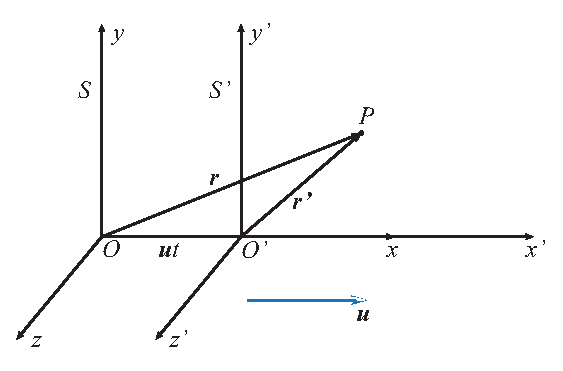
\includegraphics[scale=0.9]{C6-fig1.eps}
	\caption{伽利略坐标变换示意}
	\label{C6-fig1}
\end{figure}

先建立两个惯性系$S$, $S'$, 且$S'$相对$S$沿$S$的$x$轴正向有速度$\va*{u}$, 以$S'$系和$S'$系原点重合时作为计时起点, 即$t = t' = 0$, 那么对于空间中一点$P$有

\begin{equation}
	\va*{r} = \va*{r}' + \va*{u}t \label{C6-eq2}
\end{equation}

分量式为

\begin{equation}
	\begin{cases}
		t' = t \\
		x' = x - ut \\
		y' = y \\
		z' = z
	\end{cases}
    \label{C6-eq3}
\end{equation}


将式(\ref{C6-eq3})称为\textbf{伽利略逆变换}, 正变换即是把$x$写在左边, $x'$写在右边. 



\subsection{对伽利略变换的讨论(伽利略变换的绝对时空观)}

如果时间空间均匀, 绝对, 与参考系无关, 比如: 

\vskip 0.3cm

\begin{enumerate}
	
	\item 运动飞船中的人测一根铁棍的长度等于地面上的人测那根铁棍的长度.
	
	\item 飞船上的人看一场电影的他认为自己过去的时间应该等于地面上的人看飞船里播放的电影的他认为自己用的时间. 
	
\end{enumerate}

\vskip 0.3cm

那么伽利略变换的正确性是显然的. 因为上面这两个例子就是伽利略变换可直接推出的结果, 这种观点就称为\textbf{绝对时空观}. 

所以说\textbf{伽利略变换是与绝对时空观绑定的, 伽利略变换本身是绝对时空观的数学表达式. }

\vskip 0.3cm

归纳如下: 

\begin{figure}[htbp]
	\centering
	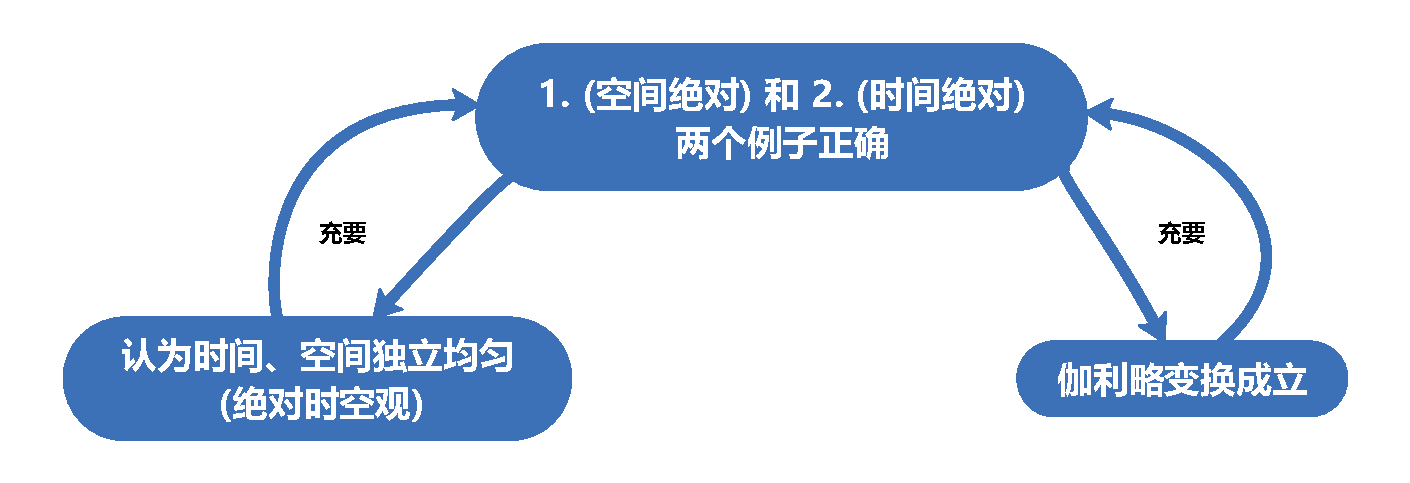
\includegraphics[scale=0.5]{C6-fig2.pdf}
	\caption{绝对时空观讨论}
	\label{C6-fig2}
\end{figure}

\subsection{伽利略相对性原理}

因为式(\ref{C6-eq3})中后三个坐标分量式恒成立, 又因为$\dd{t} = \dd{t'}$, 所以可得

\begin{equation}
	\begin{cases}
		\va*{v}'_x = \va*{v}_x - \va*{u} \\
		\va*{v}'_y = \va*{v}_y \\
		\va*{v}_z = \va*{v}_z
	\end{cases}
    \label{C6-eq4}
\end{equation}

再次求导可得

\begin{equation}
	\begin{cases}
		\va*{a}'_x = \va*{a}_x \\
		\va*{a}'_y = \va*{a}_y \\
		\va*{a}'_z = \va*{a}_z
	\end{cases}
    \label{C6-eq5}
\end{equation}

即速度和加速度的变换式. 显然\textbf{加速度有伽利略变换不变性. }

在$S$系与$S'$系分别用牛顿第二定律, 有

\begin{equation}
	\begin{cases}
		\va*{F} = m \va*{a} \\
		\va*{F}' = m' \va*{a}' 
	\end{cases}
    \label{C6-eq6}
\end{equation}

因为经典力学还认为质量是常量, 所以$\va*{F} = \va*{F}'$. 因此\textbf{牛顿定律有伽利略变换形式不变性}, 所以建立在牛顿定律上的经典力学均有伽利略变换形式不变性, 即\textbf{一切力学规律在所有惯性系中相同}(一切力学规律建立在牛顿定律上, 伽利略变换在两个惯性系间). 

\subsection{总结}

正像牛顿第二定律与动量定理, 冲量定理是相互可推证的一样, 伽利略变换本是自洽的经典力学的一块拼图, 但它却给后人留下了另一块空白. 至此, 其实只是交代的伽利略相对性原理, 也没有计算, 但这一部分对于整体理解经典力学和狭义相对论的关系有很重要的作用. 

\subsection{坏了}

先是麦克斯韦的电磁理论, 他理论推导出真空中光(电磁波)速为定值, 但因为速度无伽利略变换不变性, 这没法解释(大悲). 

然后物理学家就提出以太, 将以太作为一个绝对静止的参考系, 认为光速是相对于乙态系的. 

\begin{note}
	
	但其实这个时候就自相矛盾的, 伽利略相对性原理指出没有惯性系是特殊的, 现在人为建立了一个特殊惯性系. 
	
\end{note}

为了证明以太存在或者说光速也满足伽利略变换式, 迈克尔逊和莫雷做了以下实验: 

仪器相对地面静止, 以太绝对静止, 那么仪器相对以太有一个速度$\va*{v}$. 

\begin{figure}[htbp]
	\centering
	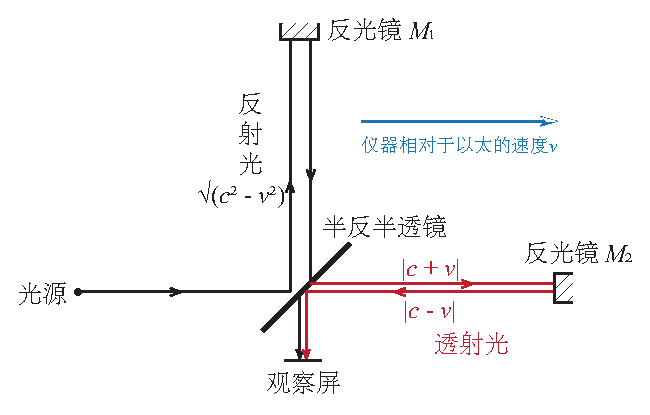
\includegraphics[scale=1.0]{C6-fig2.eps}
	\caption{迈克尔逊-莫雷实验示意}
\end{figure}

具体原理涉及到电磁波的干涉, 待各位大二上了解. 总之观察屏上应有干涉条纹且比较明显, 但结果是什么也没有, 所以经典理论遇到了困难. 

\newpage

\section{洛伦兹变换}\label{6.2}

\subsection{狭义相对论的两条基本假设}

为解决电磁学(光速$c$为定值)与经典力学(伽利略变换)间的矛盾, 爱因斯坦提出了狭义相对论的两条基本假设: 

\begin{postulate}[狭义相对论基本假设] \label{C6-po1}
	\begin{enumerate}
		
		\item 惯性系中物理定律相同(推广了伽利略的相对性原理); \label{C6-po1.1}
		
		\item 光速不变(无论如何观察光, 其速度为定值). \label{C6-po1.2}
		
	\end{enumerate}
\end{postulate}

\subsection{洛伦兹变换}

基于爱因斯坦的两条假设(\ref{C6-po1}), 可推导新的坐标变换. 

设一事件在$S$, $S'$系观察坐标为$(x, y, z, t)$, $(x', y', z', t')$. 

首先由假设 \ref{C6-po1.1} 得: 如果一个物体在$S$中不受力, 做匀速直线运动, 那么因为物理定律相同, 在$S'$系中观察其仍不受力, 还是匀速直线运动, 这就必然要有$x' = k_2x + b_1$, $y' = k_2y + b_2$, 即线性变换. 

再由假设 \ref{C6-po1.2} 得: 无论在$S$系还是$S'$系, 看一束光, 光的速度均应相同. 

最后, 因为伽利略变换的低速正确性, 这个新变换式在$\abs{\va*{u}} \ll c$时应能退化成伽利略变换. 

基于以上结论, 不妨写出以下变换式

\begin{equation}
	\begin{cases}
		x = k(x' + ut') \\
		x' = k'(x - ut)
	\end{cases}
    \label{C6-eq7}
\end{equation}

由于假设\ref{C6-po1.1}, 有$k' = k$. 将(\ref{C6-eq7})中两式相乘, 得

\begin{equation}
	xx' = k^2 (x' + ut') (x - ut) \label{C6-eq8}
\end{equation}

因为光速不变性, 我们把这个事件特殊化, 取为一束光运动到的坐标. 把$t = t' = 0$的时刻取为两惯性系重合且光从$x = x' = 0$位置射出那一刻, 那么有

\begin{equation}
	\begin{cases}
		x = ct \\
		x' = ct'
	\end{cases}
    \label{C6-eq9}
\end{equation}

代入式(\ref{C6-eq8}), 得

\begin{equation}
	k = \dfrac{c}{\sqrt{c^2 - u^2}} = \dfrac{1}{\sqrt{1 - \dfrac{u^2}{c^2}}} \label{C6-eq10}
\end{equation}

\newpage

于是

\begin{equation}
	\begin{cases}
		x = \dfrac{x' + ut'}{\sqrt{1 - \dfrac{u^2}{c^2}}} \\ \vspace{1ex}
		x' = \dfrac{x - ut}{\sqrt{1 - \dfrac{u^2}{c^2}}}
	\end{cases}
    \label{C6-eq11}
\end{equation}

两式消去$x$, $x'$分别得

\begin{equation}
	\begin{cases}
		t = \dfrac{t' + \dfrac{u x'}{c^2}}{\sqrt{1 - \dfrac{u^2}{c^2}}} \\ \vspace{2.0ex}
		t' = \dfrac{t - \dfrac{u x}{c^2}}{\sqrt{1 - \dfrac{u^2}{c^2}}}
	\end{cases}
    \label{C6-eq12}
\end{equation}

式(\ref{C6-eq11}), (\ref{C6-eq12})即为\textbf{洛伦兹变换式}, 其中用$S'$坐标描述$S$坐标的为逆变换, 反之则为正变换\footnote{正逆变换无绝对, 两者可以变换叫法. }. 

此外介绍洛伦兹速度变换: 

在$S$系, 有

\begin{equation}
	\begin{cases}
		v_x = \dfrac{\dd{x}}{\dd{t}} \\ 
		\vspace{1ex}
		v_y = \dfrac{\dd{y}}{\dd{t}} \\ \vspace{1ex}
		v_z = \dfrac{\dd{z}}{\dd{t}} 
	\end{cases}
    \label{C6-eq13}
\end{equation}

在$S'$系, 有

\begin{equation}
	\begin{cases}
		v_x' = \dfrac{\dd{x'}}{\dd{t'}} \\ 
		\vspace{1ex}
		v_y' = \dfrac{\dd{y'}}{\dd{t'}} \\ \vspace{1ex}
		v_z' = \dfrac{\dd{z'}}{\dd{t'}} 
	\end{cases}
	\label{C6-eq14}
\end{equation}

联立即得$v_x'$

\begin{equation}
	v_x' = \dfrac{\dd{x'}}{\dd{t'}} = \dfrac{\dfrac{\dd{x'}}{\dd{t}}}{\dfrac{\dd{t'}}{\dd{t}}} = \dfrac{\dfrac{x}{t} - u}{1 - \dfrac{u}{c^2} \dfrac{\dd{x}}{\dd{t}}} = \dfrac{v_x - u}{1 - \dfrac{u v_x}{c^2}} \label{C6-eq15}
\end{equation}

$v_y'$, $v_z'$同理. 

\newpage

\begin{note}
	一个记忆小技巧, 只记忆$x$和$t$的变换式, 要使用速度变换式时如此做: 
	
	\begin{equation*}
		v_x = \dfrac{x - ut}{\sqrt{1 - \dfrac{u^2}{c^2}}} / \dfrac{t - \dfrac{x c}{c^2}}{\sqrt{1 - \dfrac{u^2}{c^2}}}
	\end{equation*}
	
	两边同时除以$t$即可得到式(\ref{C6-eq15})的最后结果. 
	
\end{note}

\subsection{对于洛伦兹变换的讨论}

\begin{enumerate}
	
	\item 首先当然是要记清公式形式, 这个公式是这一部分的基础, 必须牢记. 
	
	\item 公式是在$S'$系相对$S$系有沿$x$轴正向大小为$u$的速度时推出的, 假若$S'$系相对$S$系向$x$轴负向有$u$速度, 分子上第二部分符号要取反. 同时也可能是$y$, $z$轴方向有相对速度, 要看清题意, 有相对速度的方向的速度变换式与无相对速度方向的速度变换式不同. 
	
	\item 讨论$x_1' - x_2'$的时候, 用$\frac{x_1 - ut_1}{\sqrt{1 - \frac{u^2}{c^2}}} - \frac{x_2 - ut_2}{\sqrt{1 - \frac{u^2}{c^2}}}$即可. 
	
\end{enumerate}

\vskip 0.4cm

\begin{example}
	地球上一人以10 s跑完100 m, 在速度为$0.98 c$的飞船中观察, 其用了多少时间, 跑了多远? 
	
	\begin{solution}
		
		参考图(\ref{C6-fig1}), 本题中, 将地球作为$S$系, 将飞船作为$S'$系. 
		
		本质上是已知$t_2 - t_1$, $x_2 - x_1$, 求$t_2' - t_1'$以及$x_2' - x_1'$.
		
		由于
		
		\begin{equation*}
			t_2' - t_1' = \dfrac{t_1 - \dfrac{u x_1}{c^2} - t_2 + \dfrac{u x_2}{c^2}}{\sqrt{1 - \qty(\dfrac{u}{c})^2}}
		\end{equation*}
		
		代入数据, 解得$t_2' - t_1' = 50.25$ s.
		
		同理可以求得$x_2' - x_1'$. 
		
	\end{solution}
	
\end{example}

\begin{example}
	地面上测到两飞船分别以$0.9c$, $-0.9c$的速度向相反方向飞行, 求一飞船相对另一飞船的速度. 
	
	\begin{solution}
		
		记向左飞的为\textcircled{1}, 向右飞的为\textcircled{2}.
		
		题目问的是在相对\textcircled{1}静止的参考系中观察\textcircled{2}的速度的大小, 不妨设相对\textcircled{1}和地球静止的系分别为$S$系和$S'$系, 在$S'$系, 即地球上观察\textcircled{2}的速度$v_x' = 0.9c$, 现在要求$v_x$.
		
		\begin{equation*}
			v_x = \dfrac{v_x' + u}{1 + \dfrac{u v_x'}{c^2}} = \dfrac{0.9c + 0.9c}{1 + 0.81} = 0.994c
		\end{equation*}
		
	\end{solution}
	
	\begin{note}
		
		本题有两个重点: 
		
		\begin{enumerate}
			
			\item 在理解$S$系, $S'$系和物体方面, 显然这是三个物体(系可以固连在物体上随物体运动), 因此要想套公式, 首先要分清哪个是$S$系, $S'$系和待研究物体. 
			
			\item 在一个系中观察物体, 其速度一定小于$c$, 但在一个系中观察两个物体, 他们的相对速度可以超过$c$. 
			
		\end{enumerate}
		
	\end{note}
	
\end{example}

\subsection{洛伦兹变换的意义}

$\bullet$ 揭示了空间, 时间, 物质运动间的联系. 

$\bullet$ 光速是一切运动速度的上限. 

\section{狭义相对论基础}\label{6.3}

\subsection{狭义相对论的时空观}

\subsubsection{同时性的相对性}

我们依然假设$S$, $S'$系是两个惯性系, $S'$系相对$S$系有沿$x$正方向的速度$\va*{u}$. 在$S$系测得事件1, 2的坐标为$\qty(x_1, y_1, z_1, t_1)$, $\qty(x_2, y_2, z_2, t_2)$; $S'$系测得事件1, 2坐标为$\qty(x_1', y_1', z_1', t_1')$, $\qty(x_2', y_2', z_2', t_2')$.

根据$S$系中观察的结论讨论: 

\begin{enumerate}
	
	\item $t_2 - t_1 = \Delta t = 0$, 则
	
	\begin{equation}
		t_2' - t_1' = \dfrac{\Delta t - \dfrac{u x_1}{c^2} + \dfrac{u x_2}{c^2}}{\sqrt{1 - \dfrac{u^2}{c^2}}} = \dfrac{u(x_2 - x_1)}{c^2\sqrt{1 - \dfrac{u^2}{c^2}}}
		\label{C6-eq16}
	\end{equation}
	
	若$x_2 = x_1$, 则有$t_2' - t_1' = 0$. 反之不一定, 且先后不确定. 
	
	\item $t_2 - t_1 = \Delta t \neq 0$, 则
	
	\begin{equation}
		t_2' - t_1' = \dfrac{c^2(t_2 - t_1) + u(x_2 - x_1)}{c^2\sqrt{1 - \dfrac{u^2}{c^2}}} 
		\label{C6-eq17}
	\end{equation}
	
	$t_2 - t_1$与$\frac{u(x_2 - x_1)}{c^2}$的大小关系决定了在$S'$系观察两事件的先后.
	
\end{enumerate}

因此, 对于不相关事件1, 2, 两个惯性系分别观察他们发生的先后是不太能直接认为相关的, 即$t_2 > t_1$不能直接说明$t_2'$和$t_1$的关系. 但对于因果事件, 如射击与击中, 无论如何观察, 均是射击在前, 击中在后.

\begin{example}
	有一长为600 m的列车, 其速度为$0.4c$, 地面上观察者发现有两个闪电同时击中火车前后端. 此时车上乘客测定的时间间隔为多少? 哪一端先被击中? 
	
	\begin{solution}
		
		记$t_1$为地面观察闪电击中前端的时刻, $t_2$为地面观测闪电击中后端的时刻, $t_1'$, $t_2'$意义易知.
		\begin{align*}
			x_1' - x_2' &= 600 \\
			t_1' - t_2' &= \dfrac{t_1 - t_2 - \dfrac{u x_1}{c^2} + \dfrac{u x_2}{c^2}}{\sqrt{1-0.16}} \\
			x_1 - x_2 &= \dfrac{x_1' - x_2' + u\qty(t_1' - t_2')}{\sqrt{1 - 0.16}} \\
			t_2 - t_1 &= 0
		\end{align*}
		
		解得$t_1' - t_2' = -8 \times 10^{-7}$ s, 即闪电在车上乘客看来先击中前端, 早$8 \times 10^{-7}$ s. 
		
	\end{solution}
	
\end{example}

\subsubsection{钟慢效应与尺缩效应}

\noindent \textbf{钟慢效应}

原时: 把某一个惯性系中同一地点先后发生的两个事件的时间间隔称为原时. 即在同一个惯性系同一地点用一个钟测出的时间差. 

从前面狭义相对论的“同时”的相对性的讨论知有: 

\begin{equation}
	t_2' - t_1' = \dfrac{t_2 - t_1 - \dfrac{u}{c^2} \qty(x_2 - x_1)}{\sqrt{1 - \dfrac{u^2}{c^2}}} \label{C6-eq18}
\end{equation}

由于$x_2 - x_1 = 0$, 则$t_2' - t_1' = \dfrac{\qty(t_2 - t_1)}{\sqrt{1 - \dfrac{u^2}{c^2}}} > t_2 - t_1$. 

所以说在$S'$系观察$S$系中先后发生的两件事比在S系观察先后发生的两件事用时长. 也就是一开始的例子, 在飞船中看一场电影的时间与地面上的人看飞船里这场电影时间是不同的. 

总结为: \textbf{原时最短, 任何惯性系中的观察者看别的惯性系的时间总会比本惯性系的时间慢}(相对自己静止的钟走1分, 相对自己运动的钟走1秒). 

\vskip 0.3cm

\begin{example}
    粒子寿命问题: 带静电的$\Pi$介子不稳定, 其静止寿命为$2.38 \times 10^{-8}$ s, 实验室测得一束$\Pi$介子速率为$0.99c$, 用狭义相对论计算实验人员观测出的$\Pi$介子寿命. 
	
	\begin{solution}
		\begin{equation*}
			t = \dfrac{t'}{\sqrt{1 - \dfrac{u^2}{c^2}}} = 1.772 \times 10^{-7} \textrm{~s}
		\end{equation*}
	\end{solution}
	
\end{example}

\begin{note}
	
	$t' = 2.38 \times 10^{-8}$ s是相对$\Pi$介子静止的惯性系的观测结果, 是原时
\end{note}

\vskip 0.3cm

\noindent \textbf{尺缩效应}

固有长度: 在相对被测物体静止的系中任意方式(无论是否同时)测得其首尾坐标并作差后得到的被测物体长度. 

在相对杆不静止的另一个惯性系中测量被测物体长度, 要求同时测得首尾端坐标并作差, 接下来取$S'$系相对$S$系$x$轴正向速度为$\va*{u}$, $S'$系相对被测物体静止. 

由于

\begin{align}
	x_2' - x_1' &= \dfrac{\qty(x_2 - x_1) - u\qty(t_2 - t_1)}{\sqrt{1 - \qty(\dfrac{u}{c})^2}} \label{C6-eq19} \\
	t_2 &= t_1 \label{C6-eq20}
\end{align}

所以

\begin{equation}
	x_2' - x_1' = \dfrac{x_2 - x_1}{\sqrt{1 - \qty(\dfrac{u}{c})^2}} > x_2 - x_1 \label{C6-eq21}
\end{equation}

其中, $x_2' - x_1'$为固有长度. 也就是说, 飞船中测物体长为1 m,地面上的人测飞船中这个物体长小于1 m. 

总结为: \textbf{原长最长, 沿相对运动方向的物体尺寸会收缩}. 如以下两例: 

\begin{figure}[H]
	\centering
	\begin{minipage}[t]{0.48\textwidth}
		\centering
		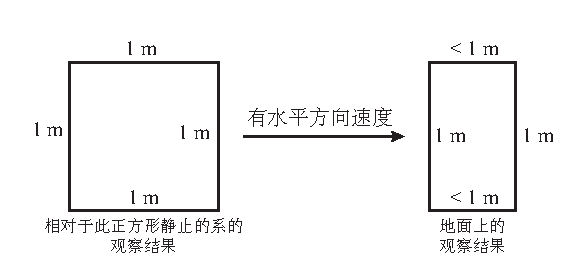
\includegraphics[scale=0.7]{C6-fig3.eps}
		\label{C6-fig3}
	\end{minipage}
	\begin{minipage}[t]{0.48\textwidth}
		\centering
		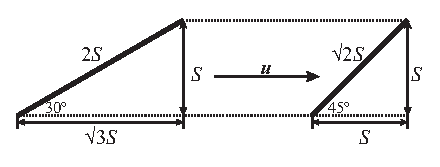
\includegraphics[scale=0.7]{C6-fig4.eps}
		\label{C6-fig4}
	\end{minipage}
\end{figure}

上右图中的$u$满足

\begin{equation*}
	\sqrt{3} S \sqrt{1 - \qty(\dfrac{u}{c})^2} = S \Rightarrow u = \dfrac{2\sqrt{3}c}{3}
\end{equation*}

\subsection{狭义相对论动力学基础}

传统的经典力学不满足洛伦兹变换, 所以要改造它, 建立相对论力学. 具体要重新定义质量、动量、能量, 使它们相应的守恒定律仍成立. 

\subsubsection{质速关系}

经典力学中有

\begin{equation}
	\va*{F} = m \va*{a} \label{C6-eq22}
\end{equation}

依照此式, $m$若不随$\va*{v}$变化, 那么只要时间足够长, 任何物体均可超越光速, 这与洛伦兹变换矛盾. 因此, 狭义相对论中给出质速关系

\begin{equation}
	m = \dfrac{m_0}{\sqrt{1 - \qty(\dfrac{u}{c})^2} \label{C6-eq23}}
\end{equation}

其中, $m_0$为本征质量(相对$m_0$静止的惯性系中测得的质量), $m$则为相对速度为$\va*{u}$的惯性系中测量得到的物体质量. 

由此得光子静止质量为0, 一切静止质量不为0的粒子速度必须小于$c$. 

进一步, 得到相对论动量和相对论动力学方程

\begin{align}
	\va*{p} &= m \va*{v} = \dfrac{m_0}{\sqrt{1 - \qty(\dfrac{u}{c})^2}} \va*{v} \label{C6-eq24} \\
	\va*{F} &= \dv{\va*{p}}{t} = \dv{t}(\dfrac{m_0}{\sqrt{1 - \qty(\dfrac{u}{c})^2}} \va*{v}) \label{C6-eq25}
\end{align}

\subsubsection{质能方程}

\begin{equation}
	E = mc^2 = \dfrac{m_0}{\sqrt{1 - \qty(\dfrac{u}{c})^2}} c^2 = m_0 c^2 + E_{\textrm{k}} = E_0 + E_{\textrm{k}} \label{C6-eq26}
\end{equation}

物体质量由动能和静止能量构成, 注意此时$E_{\textrm{k}}$不能写成$\dfrac{1}{2}mv^2$的形式. 

\vskip 0.3cm

\begin{example}
	两个静止质量$m_0$的粒子, 一个$v=0$, 另一个$v=0.6c$, 它们对心碰撞后粘在一起, 求复合粒子的静止质量. 
	\begin{solution}
		
		设合并后速度为$v'$, 静止质量为$m'$. 
		\begin{align}
			\text{动量守恒:~} \dfrac{m_0}{\sqrt{1-{(0.6)^2}}} v &= \dfrac{m'}{\sqrt{1-\dfrac{{v^2}'}{{c^2}}}} v' \label{C6-eq27} \\
			\text{能量守恒:~} m_0 {c^2} + \dfrac{m_0}{\sqrt{1-{(0.6)^2}}} {c^2} &= \dfrac{m'}{\sqrt{1 - \dfrac{{v^2}'}{{c^2}}}} {c^2} \label{C6-eq28}
		\end{align}
		
		式(\ref{C6-eq28})中消去$c^2$, 将式(\ref{C6-eq27})中$m'$用$v'$表示代入式(\ref{C6-eq28})得$v'$, 代入式(\ref{C6-eq27})得$m'$. 
		
	\end{solution}
	
\end{example}

\begin{center}
	\textcolor[RGB]{18,29,57}{\textbf{小结}}
\end{center}

本章从经典力学中的伽利略变换讲起, 说明了他与经典力学时空观的紧密联系, 再从实际实验中无法解释的现象说起, 提出狭义相对论, 并用狭义相对论创建了一套新的时空观, 一套新的动力学、能量方程. 
本章启发性很强, 题目在弄明白公式后难度不大, 本章中一些知识点在诸如《星际穿越》等科幻电影中时有出现, 对大家欣赏艺术也有帮助. 

